\section{Diagrama Entidad-Relaci\'on}

% -----------------------------------------------------------------------------
\thispagestyle{empty}
  \begin{figure}[H] \centering
    \subfloat[der]
    {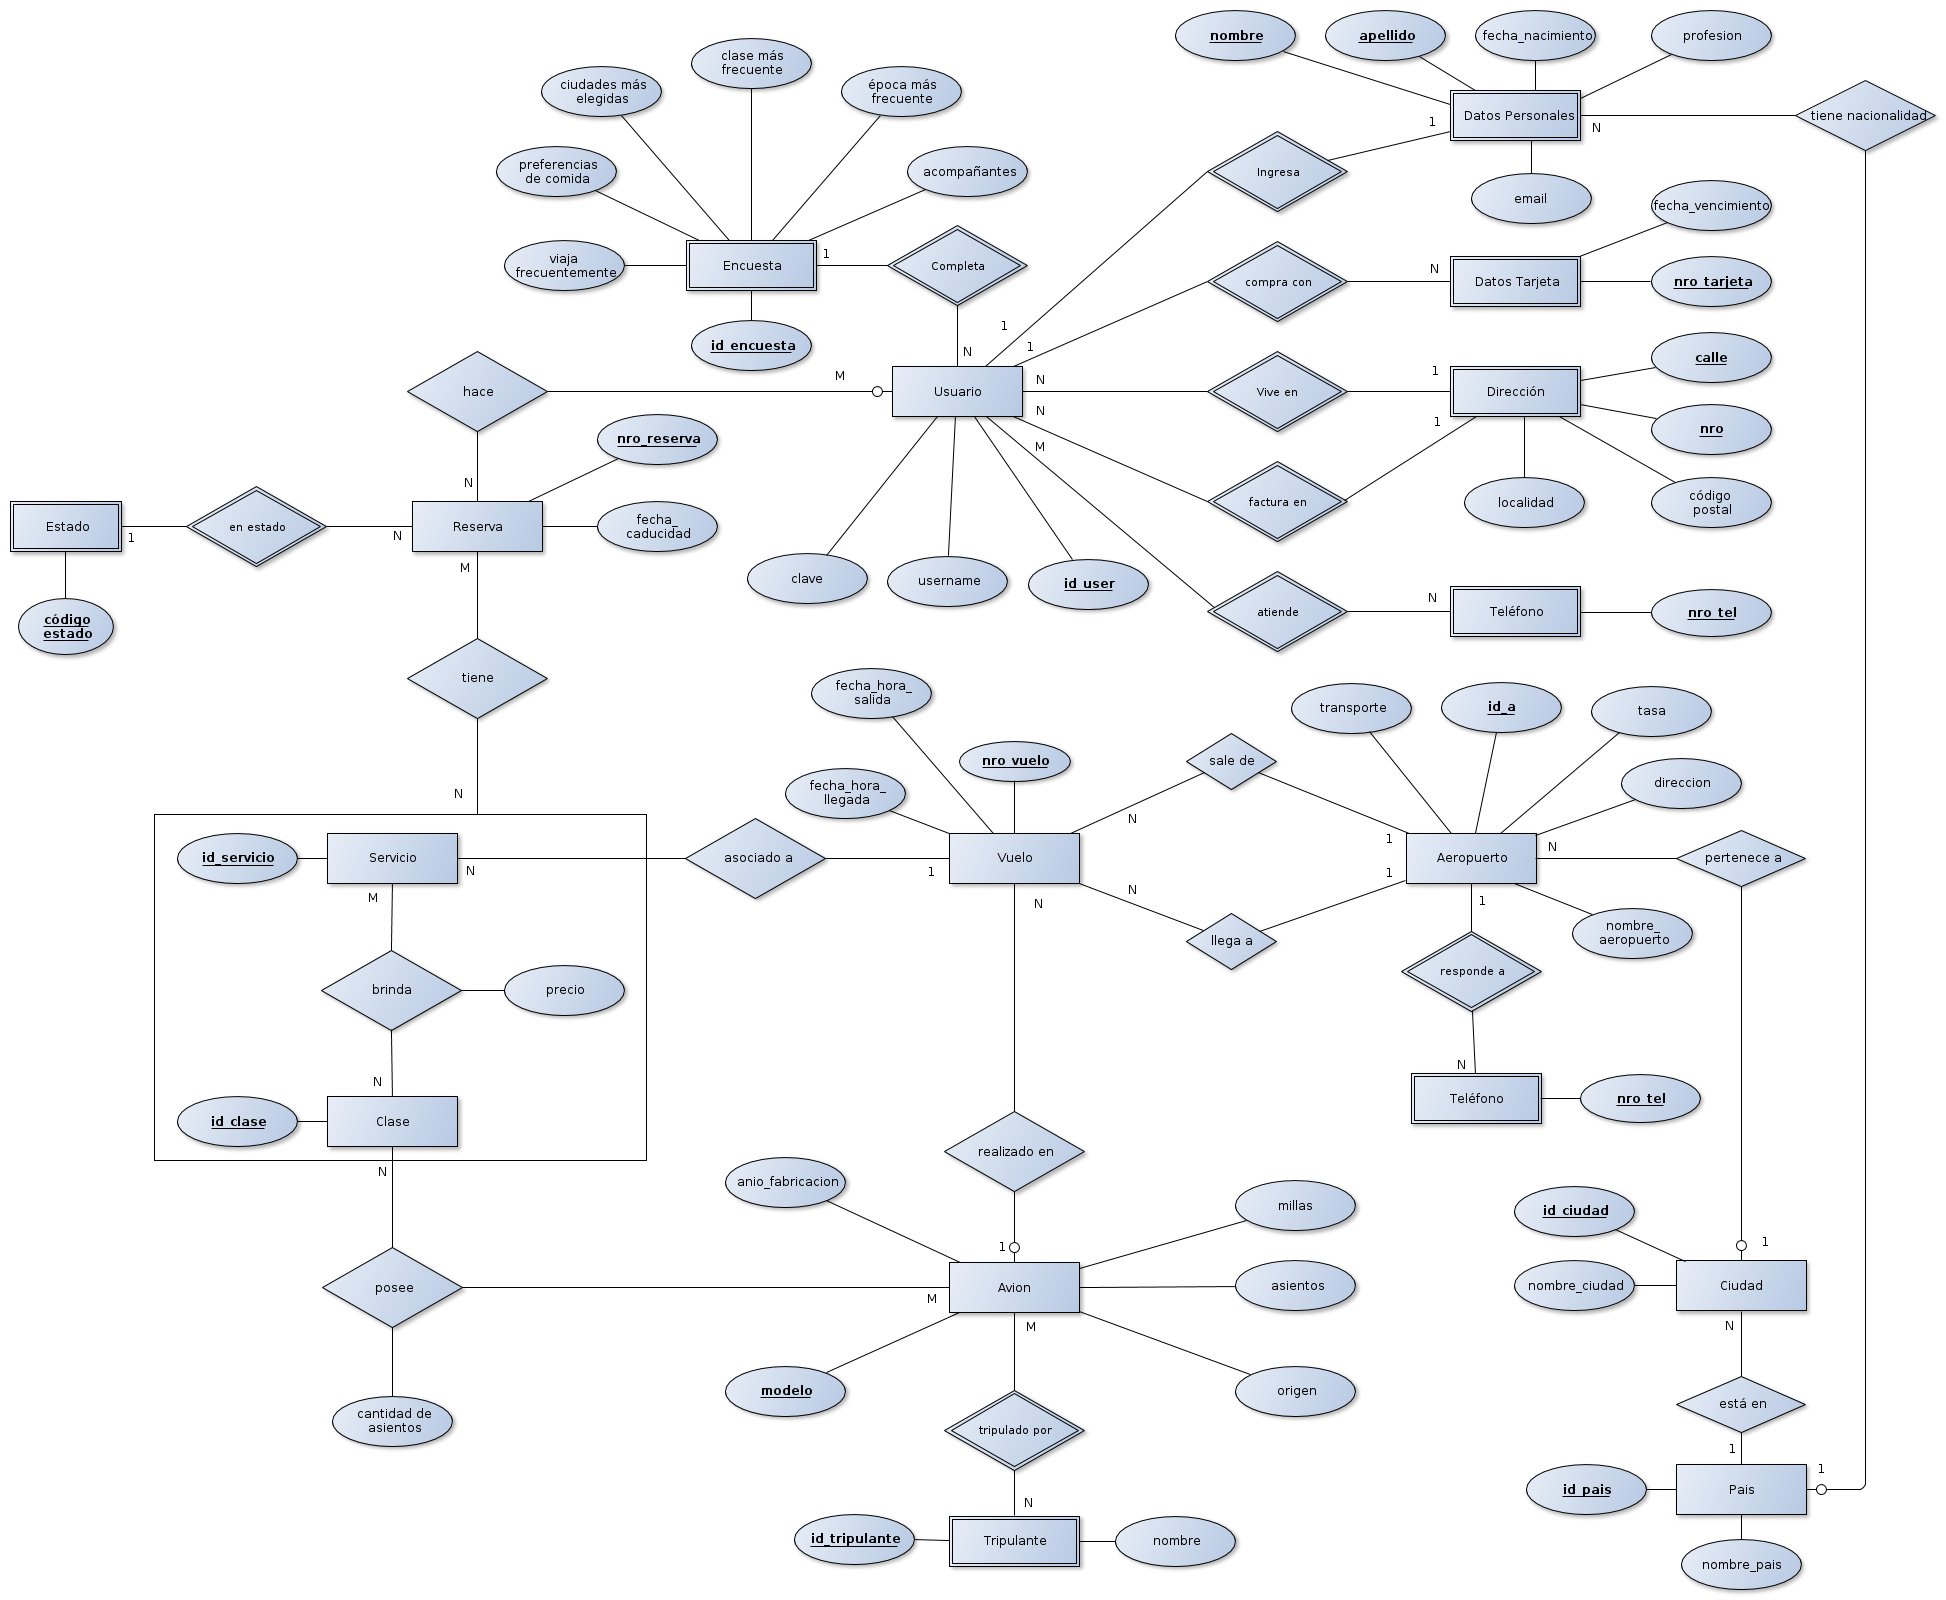
\includegraphics[width=\linewidth]{./img/der.png}}
    {}
  %\hspace*{6cm}
  \end{figure} 

% -----------------------------------------------------------------------------

\subsection{Aclaraciones y Restricciones}
  \begin{itemize}
    \item Consideramos que una reserva puede tener varios estados, estos son
          \begin{itemize}
            \item   Realizada
            \item   Cancelada
            \item   Confirmada
          \end{itemize}

          Las reservas realizadas pueden cancelarse o confirmarse.
          Es necesario confirmar una reserva para poder viajar.
          Para simplificar, suponemos que todos los usuarios con reservas
          confirmadas realizan efectivamente el viaje.
    
    \item La aerolínea ofrece servicios de viaje, y cada usuario realiza una
          reserva sobre pares de servicio-clase.
          De esta forma vemos la cantidad de asientos que está reservando por
          cada clase para un servicio.
          Cada servicio especifica la fecha y el horario del viaje. Además 
          tiene asociado un avión, que es el avión con el que se realizará
          el viaje.
          A la vez un servicio está vinculado con un vuelo. Un vuelo es
          un conjunto de servicios sin especificar. Es decir, un vuelo indica 
          que dias de la semana se brindarán servicios de un aeropuerto origen 
          a uno destino.
          Así, por ejemplo, un servicio podría ser:
          ``Un vuelo de Aeropuerto de origen Ezeiza- Buenos Aires, Aeropuerto 
          destino Newark-New Jersey el día 26/04/2013, 15:00hs, Primera Clas''.
          En cambio, un ejemplo de vuelo es:
         ``Vuelos de Aeropuerto origen Barajas-Madrid, Aeropuerto destino 
          JFK-New York, los días martes y jueve''.
	
    \item Consideramos que los mensajes que el sistema le envía a los usuarios
          no son lo suficientemente relevantes para el problema que queremos
          modelar.
          
    \item Una reserva que se encuentra en estado Realizada, está asociada con un
    	  servicio cuya fecha y hora de salida es anterior a la fecha actual.
    	  
	\item La suma de la cantidad de asientos por clase en un avión (en la 
		  interrelación se distribuyen en) es igual a lo que indica el 
		  atributo asientos de la entidad avión.
	
	\item Este modelo no contempla la posibilidad de que la aerolinea cancele un
		  vuelo. Con lo cual todo vuelo existente es efectuado.
            
  \end{itemize}